\documentclass[12pt, a4papre]{article}
\usepackage[catalan]{babel}
\usepackage[unicode]{hyperref}
\usepackage{amsmath}
\usepackage{amssymb}
\usepackage{amsthm}
\usepackage{xifthen}
\usepackage{siunitx}
\usepackage{xcolor}
\usepackage{float}
\usepackage{listings}
\usepackage{setspace}
\usepackage{graphicx}
\usepackage{tikz,lipsum,lmodern}
\usepackage[most]{tcolorbox}
\usepackage{circuitikz}
\usepackage{indentfirst}
\usepackage{verbatimbox}
\definecolor{mygreen}{RGB}{28,172,0} % color values Red, Green, Blue
\definecolor{mylilas}{RGB}{170,55,241}
\graphicspath{ {./images/} }

\hypersetup{
    colorlinks = true,
    linkcolor = blue
}

\author{	
		Igor Yuziv\\
		Gabriel\\
		Oriol\\
		Albert Tomas\\
		Daniel Vilardell}
\newpage

\title{\textbf{\textcolor{blue}{ENTIC-lab\\
	Answers to WP questions}}}
\date{2020}

\begin{document}

	\lstset{language=Matlab,%
		frame=single,  
    		%basicstyle=\color{red},
    		breaklines=true,%
    		morekeywords={matlab2tikz},
    		keywordstyle=\color{blue},%
    		morekeywords=[2]{1}, keywordstyle=[2]{\color{black}},
   		 identifierstyle=\color{black},%
    		stringstyle=\color{mylilas},
    		commentstyle=\color{mygreen},%
    		showstringspaces=false,%without this there will be a symbol in the places where there is a space
    		numbers=left,%
    		numberstyle={\tiny \color{black}},% size of the numbers
    		numbersep=9pt, % this defines how far the numbers are from the text
    		emph=[1]{for,end,break},emphstyle=[1]\color{red}, %some words to emphasise
    		%emph=[2]{word1,word2}, emphstyle=[2]{style},    
	}
	
	\maketitle
	\newpage

	\textcolor{blue}{Question 3.1:} \textbf{Which pressure increase will be observed at 3 m depth?}
	\[
		0.986\cdot\frac{3}{10} = 0.2958 Atm
	\]

	\textcolor{blue}{Question 3.2:} \textbf{Will this pressure depend or not on the atmospheric pressure at water surface? Why?}\\
	
		If what we want is to calculate the real pressure that will be exerted on the ROUV, we must also take into account the atmospheric pressure on the surface. On the other hand, if what we want is only to calculate the increase with respect of this, it will not be necessary.\\\\
	
	\textcolor{blue}{Question 3.3:} \textbf{Analyse the circuit of Fig. 4.2 and obtain the output voltage VS. Then, find the dependence of VS on the relative variation due to deformation (x) and on the power supply voltage (V). }
	\[
	\frac{V-V_{1}}{R_{o}( 1+x)} =\frac{V_{1}}{R_{0}( 1-x)} \qquad \qquad \frac{V-V_{1}}{( 1+x)} =\frac{V_{1}}{( 1-x)} 
	\]\[
	\frac{V-V_{2}}{R_{o}( 1-x)} =\frac{V_{2}}{R_{o}( 1+x)}\qquad \qquad \frac{V-V_{2}}{( 1-x)} =\frac{V_{2}}{( 1+x)} 
	\]\[
	( V-V_{1})( 1-x) =V_{1}( 1+x)
	\]\[
	( V-V_{2})( 1+x) =V_{2}( 1-x)
	\]
	Now we isolate $V_{1}$ and $V_{2}$ :
	
	\[
	V_{1} =\frac{V( 1-x)}{2}
	\qquad \qquad
	V_{2} =\frac{V( 1+x)}{2}
	\]\[
	V_{s} =V_{2} -V_{1} \ so\ Vs=-V\cdotp x
	\]
	
	\textcolor{blue}{Question 3.4:} \textbf{The datasheet of the sensor is available in Atenea. Identify there the full scale output, and then deduce the sensor sensitivity and its value when the supply voltage is not 10 V but 5 V.}\\
	
	Sensor sensitivity is $O=V\cdotp P$. So when we have 2 voltages $O_{1} =V_{1}\cdot P$ and $O_{2} =V_{2} \cdot P$

	We consider the same P for both inputs \\
	\[\frac{V_{1}}{V_{2}} =\frac{O_{1}}{O_{2}}\]
	\[O_{2} =\frac{O_{1} \cdotp V_{2}}{V_{1}} =\frac{5\cdotp 0,410}{10} =0,2V\]

	\textcolor{blue}{Question 3.5:} \textbf{What output voltages V0 will provide the sensor at the water surface (at P=100 kPa) and at 3 m depth? }

	\[V_{s} =O\cdotp P=0,2\cdotp 100k= 20mV\]
	\[V_{_{3m}} =0,2\cdotp 130k=26mV\]
	
	
	\textcolor{blue}{Question 3.6:} \textbf{ In a real case and due to changing atmospheric conditions, the pressure at the water surface can be different than 100 kPa, discuss how you could fix such effect and obtain the correct pressure data.} 
	
	To solve this problem, we are going to measure the atmospheric pressure in the laboratory so that we avoid errors.\\
	
	\textcolor{blue}{Question 3.7:}\textbf{Analyse the circuit of Fig. 4.4 and obtain its gain expression V0/(V2-V1) when R1/R2=R4/R3.  Identify the role of Rg as a gain trimmer without compromising the R1-R4 resistance matching.}
	
	\[V_{1} \cdotp G_{1} +\ ( V_{1} -V_{2}) \cdotp G_{g} +( V_{1} -Vx) =0\]
	\[( V_{2} -Vx) \cdotp G_{3} +( V_{2} -V_{1}) \cdotp G_{g} +( V_{2} -V_{o}) \cdotp G_{4} =0\]
	\[( V_{2} \cdotp G_{3} \cdotp G_{g}) -V_{1} \cdotp G_{3} \cdotp ( G_{1} +G_{2} +G_{g}) =\]
	\[=( V_{0} \cdotp G_{2} \cdotp G_{4}) +( V_{1} \cdotp G_{g} \cdotp G_{2}) -G_{2} \cdotp V_{2} \cdotp ( G_{3} +G_{4} +G_{g})\]
	
	Let's assume $G_{2} \cdotp G_{4} =G_{1} \cdotp G_{3}$, then we isolate:
	\[V_{0}  = \frac{V_{2} -V_{1} \cdotp ( G_{3} \cdotp G_{g} +G_{2} \cdotp G_{3} +G_{2} \cdotp G_{g} +G_{4} \cdotp G_{2})}{G_{2} \cdotp G_{4}}\]
	\[\frac{V_{0}}{V_{2} -V_{1}} =1+\frac{R_{1} -R_{4}}{R_{g}} +\frac{R_{4}}{R_{3}}\]
	\\
	
	\textcolor{blue}{Question 3.8:} \textbf{Compare this result with the gain expression provided by the manufacturer using the resistor values shown in the INA126 datasheet.}\\
	\[
		G=5+\frac{80k\si{\ohm}}{R_{g}}
	\]
	\[
		R_{4} =R_{1} =40k\si{\ohm}\qquad
		R_{2} =R_{3} =10k\si{\ohm}
	\]

	\textcolor{blue}{Question 3.9:}\textbf{ Identify the saturation voltage of the amplifier}
	\[
		5 V - 0,75 V = 4,25 V = V_{sat}
	\]

	\textcolor{blue}{Question 3.10:} \textbf{Which amplifier gain is necessary to obtain the maximum amplifier voltage output for 3m depth? Which Rg resistor value will provide this gain?}
	
	\[
		G = \frac{v_{sat}}{v_{in}} = \frac{4.25}{26} = 163.46
	\]
	\[
		R_g = \frac{80}{163.46-5} = \SI{504.86}{\ohm} \approx \SI{510}{\ohm}
	\]
	\\
	\textcolor{blue}{Question 3.11:} \textbf{Draw the sensor+amplifier schematic using the CAD schematic software} \textcolor{blue}{https://www.tinycad.net/}
	
	FALTA ESQUEMA\\
	\newpage
	\textcolor{blue}{Question 3.12:} \textbf{Obtain in the lab 10 measurement points along the measurement range. Draw its graphical representation, calculate and plot the linear regression and the linearity error (lineal regression straight line – measured points). }
	
	\begin{table}[H]
	\centering
	\begin{tabular}{||c c ||} 
	 \hline
		 Preassure[Atm] & Voltage[$V$] \\ [0.5ex] 
	 \hline\hline
	 	0 		& 1.96 \\
		 0.1 		& 1.97  \\ 
		 0.15 	& 1.98  \\ 
		 0.2 		&  1.99\\
		 0.25 	& 1.995  \\ 
		 0.3 		& 2.00 \\
		 0.35 	& 2.003  \\ 
		 0.4 		& 2.01 \\
		 0.45 	& 2.013  \\ 
		 0.5 		& 2.019 \\ [1ex] 
	 \hline
	\end{tabular}
	\caption{Voltage output respect to Preassure input}
	\end{table}
	
	
	\begin{figure}[H]
		\begin{center}
		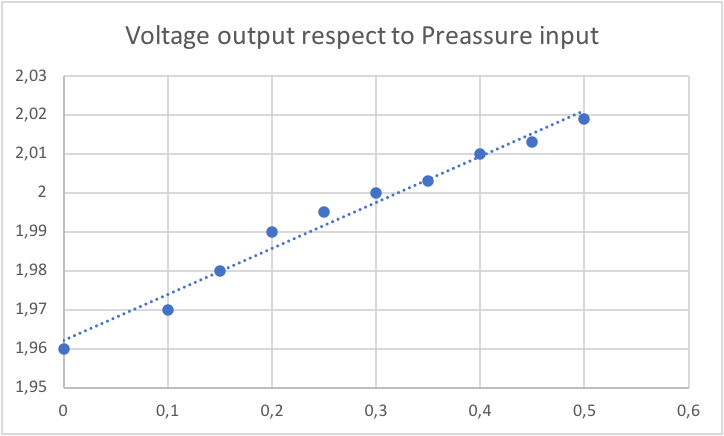
\includegraphics{ExcelGraph2.png}
	\end{center}
	\end{figure}
	
	\begin{figure}[H]
		\begin{center}
		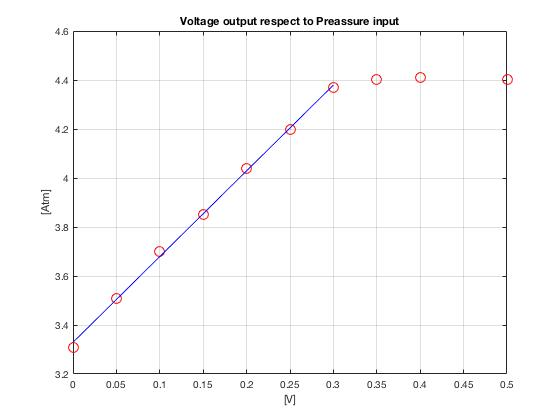
\includegraphics[width=105mm]{MatlabGraph1.jpg}
	\end{center}
	\end{figure}
	
	\lstinputlisting{codiMatlab.m}
	

	\textcolor{blue}{Question 3.13:}  \textbf{Calculate the digital data range provided by the acquisition circuit in measurements from 0 to 3m of water depth. Consider that the 10 bit A/D converter of the Arduino assigns 0 to a 0V input and 1023 (210-1) to a 5V input.}
	
	The expected values from the arduino measurement acquisition should be inside the interval
	\[
		[\frac{V_0}{5}\cdot1023, \frac{V_{0.3}}{5}\cdot1023] = [\frac{1.96}{5}\cdot1023, \frac{2.00}{5}\cdot1023] = [401.0,409.2]
	\]
	
	\textcolor{blue}{Question 3.14:} \textbf{Explain briefly what is the purpose of the following functions, used in the sketch of Fig. 4.5: Serial.begin(), analogRead(), Serial.println() and delay(). }
	\begin{itemize}
		\item \textbf{Serial.begin():} Sets the data rate in bits per second for serial data transmission.
		\item \textbf{analogRead():} Reads the value from the specified analog pin.
		\item \textbf{Serial.println():} Prints data to the serial port and skip the line.
		\item \textbf{delay():} Pauses the program for the amount of time specified as parameter.
	
	\end{itemize}


	\textcolor{blue}{Question 3.15:}  \textbf{While acquiring measures with the Arduino, smoothly increase the pressure to simulate a depth change from 0 m to 3 m. Do the measurement results displayed on the serial monitor match with the theoretical ones obtained in Question 3.13? If not, explain why. NOTE: If you are at home, use the potentiometer or the temperature sensor instead of the pressure sensor.}

	\begin{table}[H]
	\centering
	\begin{tabular}{||c c ||} 
	 \hline
		 Preassure[Atm] & Arduino output \\ [0.5ex] 
	 \hline\hline
	 	 0 		& 391  \\
		 0.1 		& 392  \\ 
		 0.15 	& 392  \\ 
		 0.2 		& 393  \\
		 0.25 	& 394  \\ 
		 0.3 		& 395  \\
		 0.35 	& 396  \\ 
		 0.4 		& 397  \\
		 0.45 	& 399  \\ 
		 0.5 		& 399  \\ [1ex] 
	 \hline
	\end{tabular}
	\caption{Arduino output respect to Preassure input}
	\end{table}
	
	FALTA EXPLICAR PERQUE NO ES IGUAL A LA PREGUNTA 3.13\\

	\textcolor{blue}{Question 3.16:} \textbf{Include a picture of the initial and final Gantt diagrams of WP3, making a reflexion about the progress and explaining any delay in the development of the tasks. }
	
	ES FA AL ACABAR LA PART\\
	Hola que tal
	
\end{document}